\documentclass{beamer}

\usepackage{polski}
\usepackage[utf8]{inputenc}
\usepackage{color}
\usepackage{amsfonts}	% Real

\usepackage{booktabs} % eleganckie tabelki


\usetheme{boxes}      % Wybór tematu wyglądu, gdy chcemy inny
%\usecolortheme{rose}   % Wybór tematu kolorystycznego, j.w.

%Konfiguracja dla pakietu hyperref:
\hypersetup{
  unicode=true,           % włączenie wyświetlania pliterek w zakładkach
%  pdfpagemode=FullScreen, % włączenie trybu pełnoekranowanego
  pdfsubject=Graph Neural Networks,      % temat prezentacji
  pdfkeywords={gnn, graph neural network, graph, classification} % slowa kluczowe
}

%% Dane do strony tytułowej
\author{Aleksy Barcz} 
\title{Graph Neural Networks\\(Scarselli, 2009)}
%\date{\today}
%\institute{Institute of Computer Science \\ Warsaw University of Technology}

\setbeamercovered{transparent}

\begin{document}
\frame{\titlepage}

\begin{frame}
\frametitle{Cechy GNN}
\begin{itemize}
	\item Klasyfikator dowolnych grafów (niepozycyjne, cykle)
	\item Klasyfikacja węzłów i klasyfikacja grafów
	\item Oparty na FNN
	\item Proste rozwiązanie problemu cykli
\end{itemize}
\end{frame}

\begin{frame}
\frametitle{Cel implementacji}
\begin{itemize}
	\item Sprawdzenie działania GNN i identyfikacja kluczowych parametrów
	\item Utworzenie wygodnego i uniwersalnego środowiska
	\item Wybrana platforma implementacji : Octave
\end{itemize}
\end{frame}

\begin{frame}
\frametitle{Format reprezentacji grafu}
\begin{itemize}
	\item \emph{nodes.csv} (etykiety węzłów):\\każdy wiersz = $l_n$; ($|l_n| \geq 1$)
	\item \emph{edges.csv} (etykiety krawędzi $x_u \Rightarrow x_n$):\\każdy wiersz = $id_u, id_n, l_{un};$
	\\($id_n$ : indeks węzła $n$ w pliku nodes.csv)\\($l_{un}$ : etykieta krawędzi, $|l_{un}| \geq 0$)
	\item \emph{output.csv} (oczekiwane wyjścia węzłów lub grafu):\\każdy wiersz = $o_n$; ($|o_n| \geq 1$)\\lub\\pojedynczy wiersz = klasa grafu
\end{itemize}
\end{frame}

\begin{frame}
\frametitle{Koncepcja GNN}
\begin{itemize}
	\item Pojedyncza sieć dla wszystkich grafów należących do problemu
	\item Dla każdego węzła automatycznie budowana reprezentacja: $x_n = f(...)$
	\item Klasyfikacja węzła: $o_n = g(x_n)$
	\item Dla zagadnienia klasyfikacji grafów, wybieramy wierzchołek reprezentujący graf
\end{itemize}
\end{frame}

\begin{frame}
\frametitle{Składowe GNN}
\begin{itemize}
	\item Dwie jednostki obliczeniowe : $f_w$ i $g_w$
	\item Wszystkie instancje $f_w$ współdzielą wagi
	\item Wszystkie instancje $g_w$ współdzielą wagi
	\item Instancje $f_w$ połączone w metasieć odwzorowującą połączenia w grafie
\end{itemize}
\end{frame}

\begin{frame}
\frametitle{Budowanie stanu węzła - $f_w$}
\begin{columns}
	\begin{column}{0.2\textwidth}
		\begin{center}
			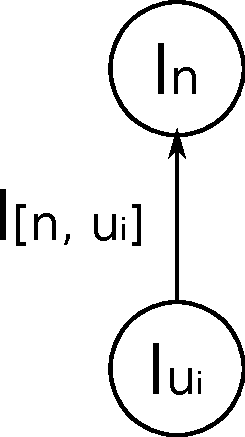
\includegraphics[scale=0.4]{img/connection}
		\end{center}
	\end{column}
	\begin{column}{0.8\textwidth}
		\begin{center}
			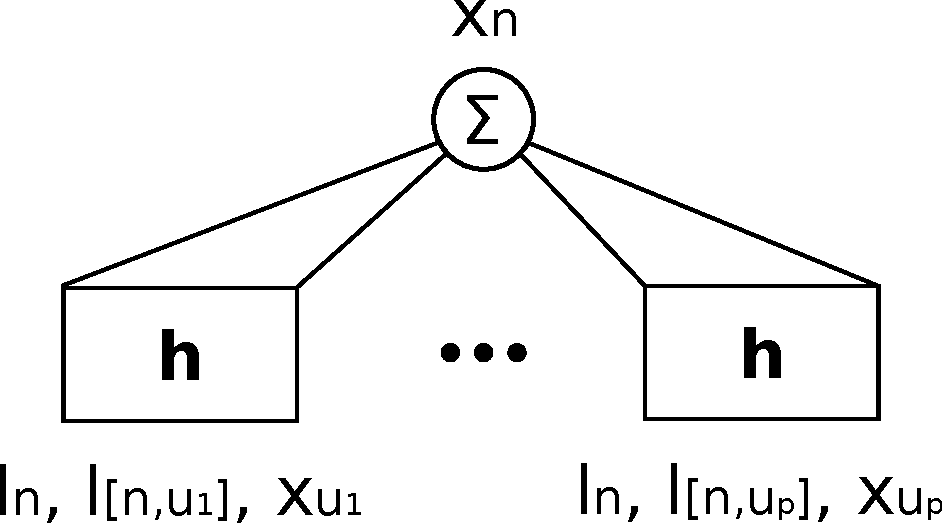
\includegraphics[scale=0.4]{img/f}
		\end{center}
	\end{column}
\end{columns}
\medskip
\begin{itemize}
	\item dla węzła $n$ rozpatrywani wszyscy sąsiedzi $u$ (krawędź $u \Rightarrow n$)
	\item $h_w$ : FNN (wejścia, warstwa $tanh$, warstwa $tanh$)
\end{itemize}
\end{frame}

\begin{frame}
\frametitle{Klasyfikacja węzła - $g_w$}
\begin{center}
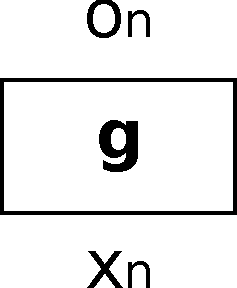
\includegraphics[scale=0.4]{img/g}
\end{center}
\begin{itemize}
	\item wejściem $g_w$ jest stan węzła $n$ : $x_n$, wyznaczony przez $f_w$
	\item $g_w$ : FNN (wejścia, warstwa $tanh$, warstwa dowolna)
\end{itemize}
\end{frame}

\begin{frame}
\frametitle{Postać globalna}
\begin{itemize}
	\item $X = {x_1, .., x_m}$ : stan - reprezentacja wszystkich węzłów grafu
	\item $F_w(X)$ : globalna funkcja przejścia
	\item $G_w(X)$ : globalna funkcja wyjścia
\end{itemize}
\end{frame}

\begin{frame}
\frametitle{Schemat uczenia GNN}
\begin{enumerate}
	\item Losowa inicjalizacja wag $h_w$ i $g_w$
	\item do osiągnięcia kryterium stopu:
	\begin{itemize}
		\item losowa inicjalizacja stanu $X$
		\item FORWARD : obliczanie $X = F_w(X)$ aż do osiągnięcia punktu stałego
		\item BACKWARD : obliczenie $G_w(X)$ i propagacja wsteczna błędu
		\item aktualizacja wag $f_w$ i $g_w$
	\end{itemize}
\end{enumerate}
\end{frame}

\begin{frame}
\frametitle{Przykładowy graf}
\begin{center}
	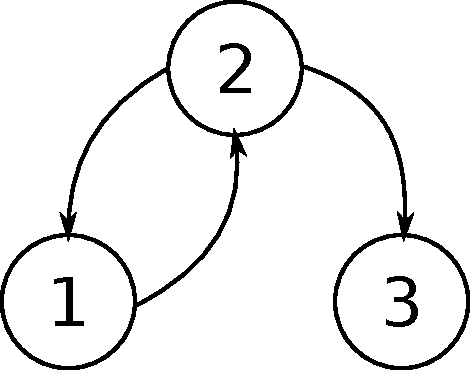
\includegraphics[scale=0.4]{img/graph}
\end{center}
\end{frame}

\begin{frame}
\frametitle{Forward - budowanie stanu}
\begin{columns}
	\begin{column}{0.66\textwidth}
		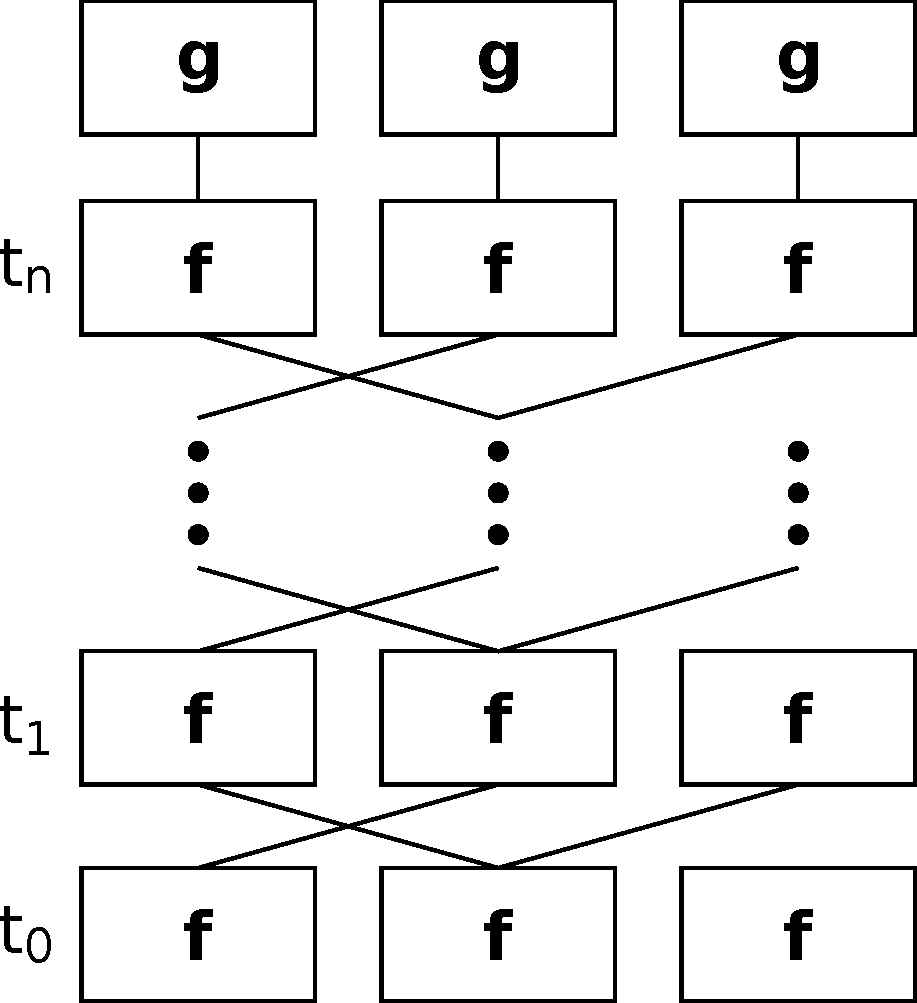
\includegraphics[scale=0.4]{img/forward}
	\end{column}
	\begin{column}{0.34\textwidth}
		\begin{itemize}
			\item BPTT
			\item $minStateDiff$
		\end{itemize}
	\end{column}
\end{columns}
\end{frame}

\begin{frame}
\frametitle{Backward - propagacja wsteczna błędu}
\begin{columns}
	\begin{column}{0.66\textwidth}
		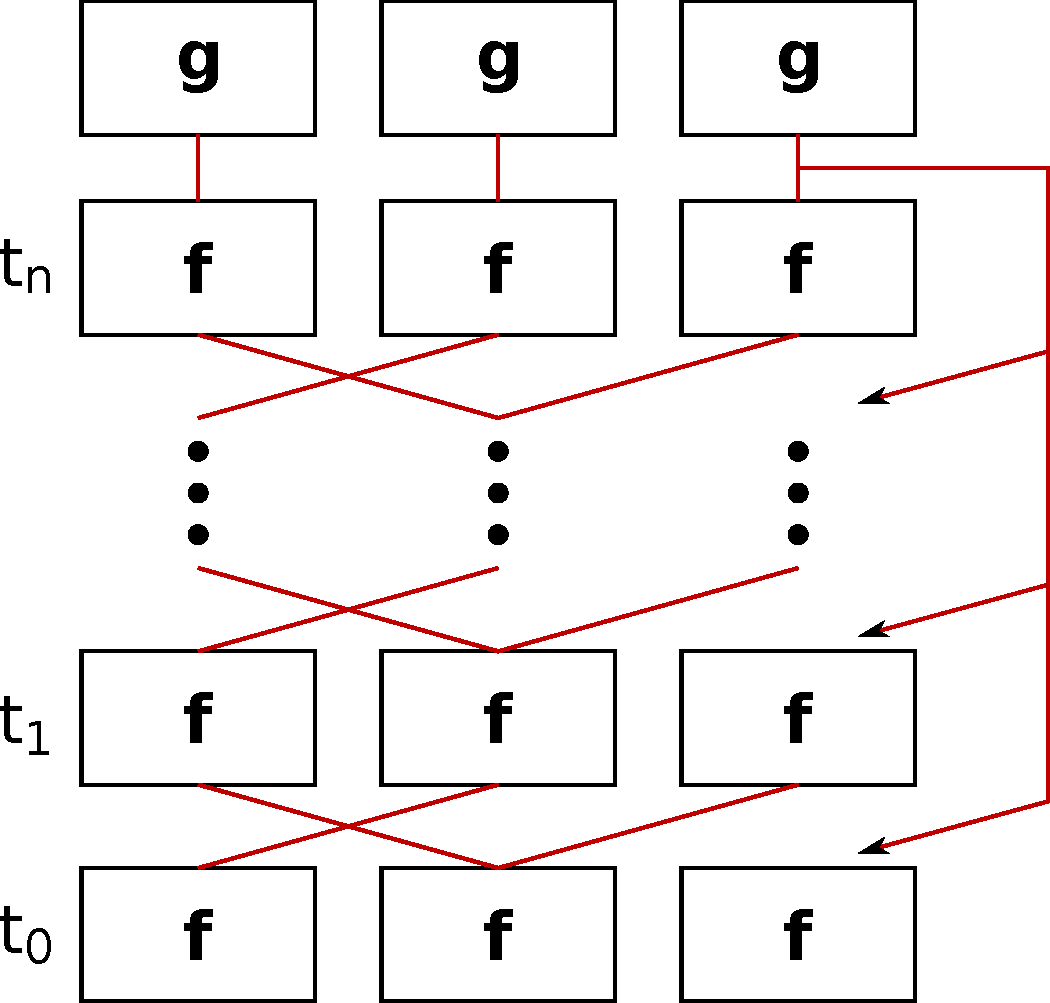
\includegraphics[scale=0.4]{img/backward}
	\end{column}
	\begin{column}{0.34\textwidth}
		\begin{itemize}
			\item Almeida-Pineda
			\item $minErrorDiff$
		\end{itemize}
	\end{column}
\end{columns}
\end{frame}

\begin{frame}
\frametitle{Własności $F_w$ (tw. Banacha)}
\begin{itemize}
	\item kontrakcja : $||F_w(X_1) - F_w(X_2)|| \leq ||X_1 - X_2||$
	\item posiada dokładnie jeden punkt stały
	\item zbieżność $F_w$ niezależna od punktu początkowego
	\item zbieżność wykładnicza - potrzebna bardzo mała ilość powtórzeń (ok. 5 do 15)
	\item jak zapewnić by $F_w$ była kontrakcją?
\end{itemize}
\end{frame}

\begin{frame}
\frametitle{Aktualizacja wag $f_w$ i $g_w$}
\begin{itemize}
	\item Kara za brak kontrakcji dla wag $f_w$
	\item $contractionConstant$
	\item Duże różnice skali między karą a oryginalną korektą
	\item RPROP
	\item $deltaMax$
\end{itemize}
\end{frame}

\begin{frame}
\frametitle{Zbiór danych}
\begin{itemize}
	\item Wykrywanie podgrafu
	\item Podobny do zbioru Scarselli
	\item 6 węzłów, 3 węzły podgrafu, $p_{edge} = 0.8$ (zamiast 0.2)
	\item Etykiety węzłów 0..10
	\item Szum Gaussowski średnia=0 std=0.25
	\item 20 grafów
\end{itemize}
\end{frame}

\begin{frame}
\frametitle{Parametry modelu - stałe}
FNN - zgodne z zaleceniami:
\begin{itemize}
	\item liczba neuronów ukrytych $h_w$ : 5
	\item liczba neuronów ukrytych $g_w$ : 5
	\item rozmiar stanu $x_n$ : 5
\end{itemize}
RPROP - zgodne z zaleceniami:
\begin{itemize}
	\item $initialDelta$ : 0.1
	\item $minDelta$ : 10e-6
	\item $maxDelta$ : 1.0 (zalecana wartość alternatywna)
	\item $factor+$ : 1.2
	\item $factor-$ : 0.5
\end{itemize}
\end{frame}

\begin{frame}
\frametitle{Parametry modelu - modyfikowane}
Zależne od problemu:
\begin{itemize}
	\item $minStateDiff$ : 10e-8 .. 10e-5
	\item $minErrorDiff$ : jw.
	\item $contractionConstant$ : 0.5 .. 1.2
\end{itemize}
\end{frame}

\begin{frame}
\frametitle{Eksperymenty}
Legenda:
\begin{itemize}
	\item $nForward$ : ilość kroków procedury budowania stanu (przerywana po przekroczeniu 200)
	\item $nBackward$ : ilość kroków akumulacji błędu (Almeida-Pineda, przerywane po przekroczeniu 200)
	\item $penalty$ : czy na którąkolwiek z wag została nałożona kara kontrakcji?
	\item \emph{de/dw influence} : procent korekt wag zgodnych znakiem z gradientem błędu
	\item \emph{dp/dw influence} : procent korekt wag zgodnych znakiem z pochodną kary kontrakcji
\end{itemize}
\end{frame}

\begin{frame}
\frametitle{Eksperyment 1 : wpływ początkowych wartości wag}
\begin{itemize}
	\item 10 grafów
	\item 9 sieci GNN o losowych wagach
	\item $contractionConstant$ = 0.9
	\item $minStateDiff$ = 10e-08
	\item $minErrorDiff$ = $minStateDiff$
\end{itemize}
\end{frame}

\begin{frame}
	\includegraphics[scale=0.065]{img/rmse_gnn1-9}
\end{frame}
\begin{frame}
	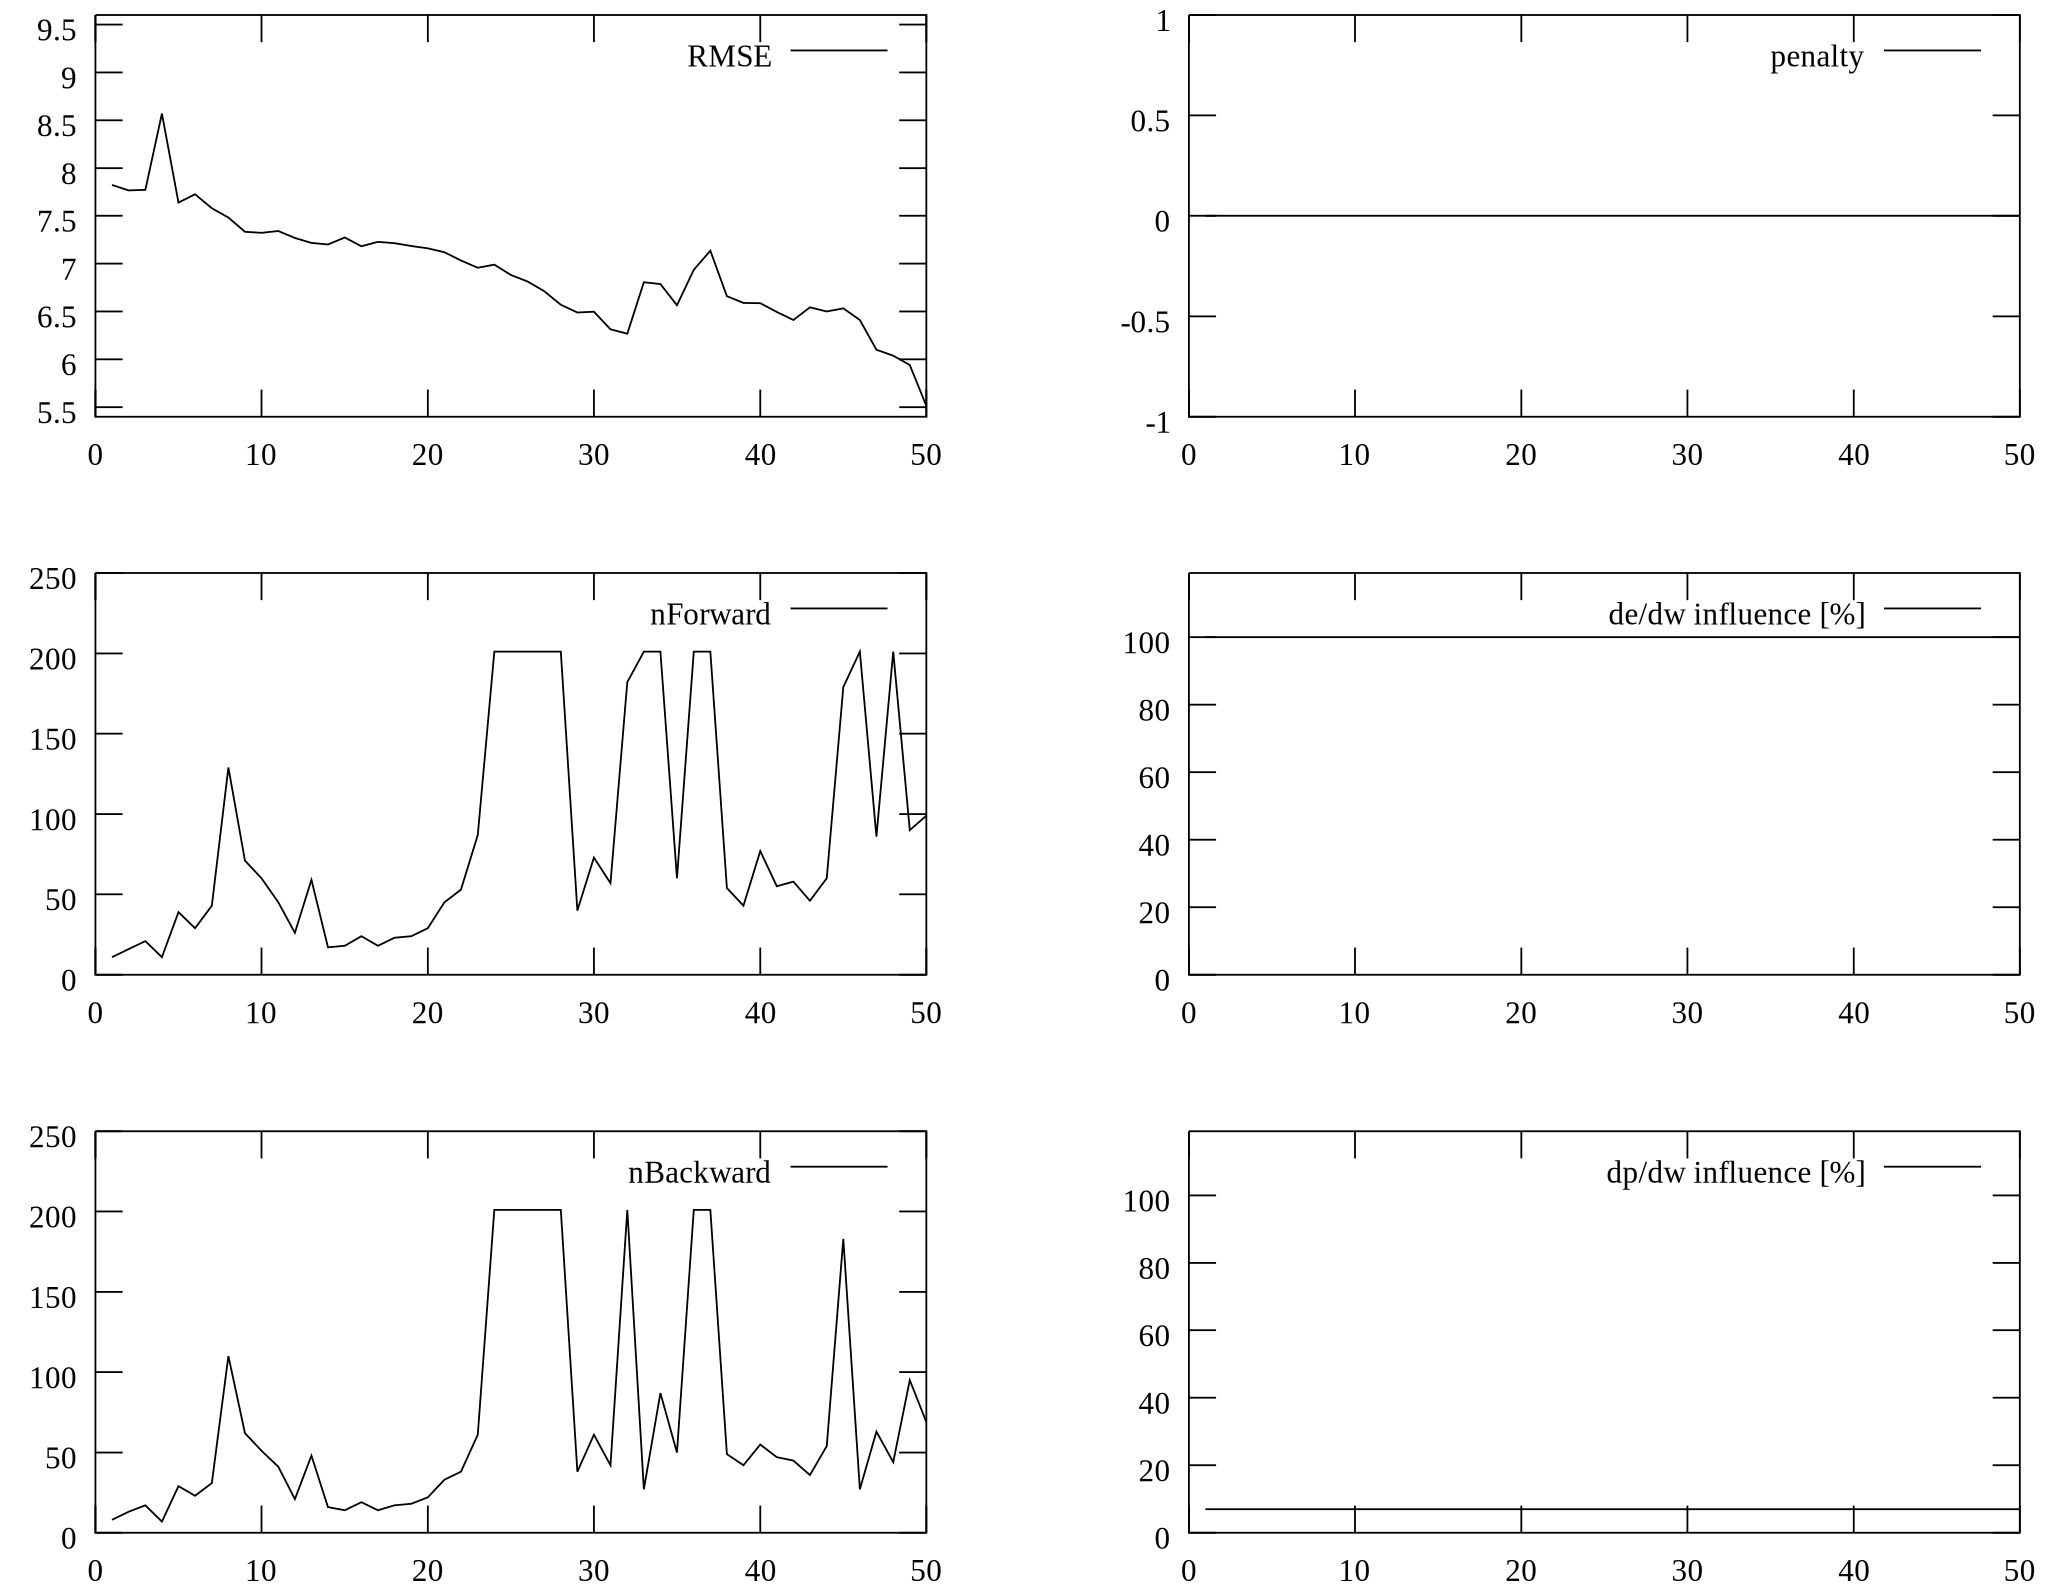
\includegraphics[scale=0.065]{img/gnn5}
\end{frame}
\begin{frame}
	\includegraphics[scale=0.065]{img/gnn7}
\end{frame}
\begin{frame}
	\includegraphics[scale=0.065]{img/gnn1}
\end{frame}
\begin{frame}
	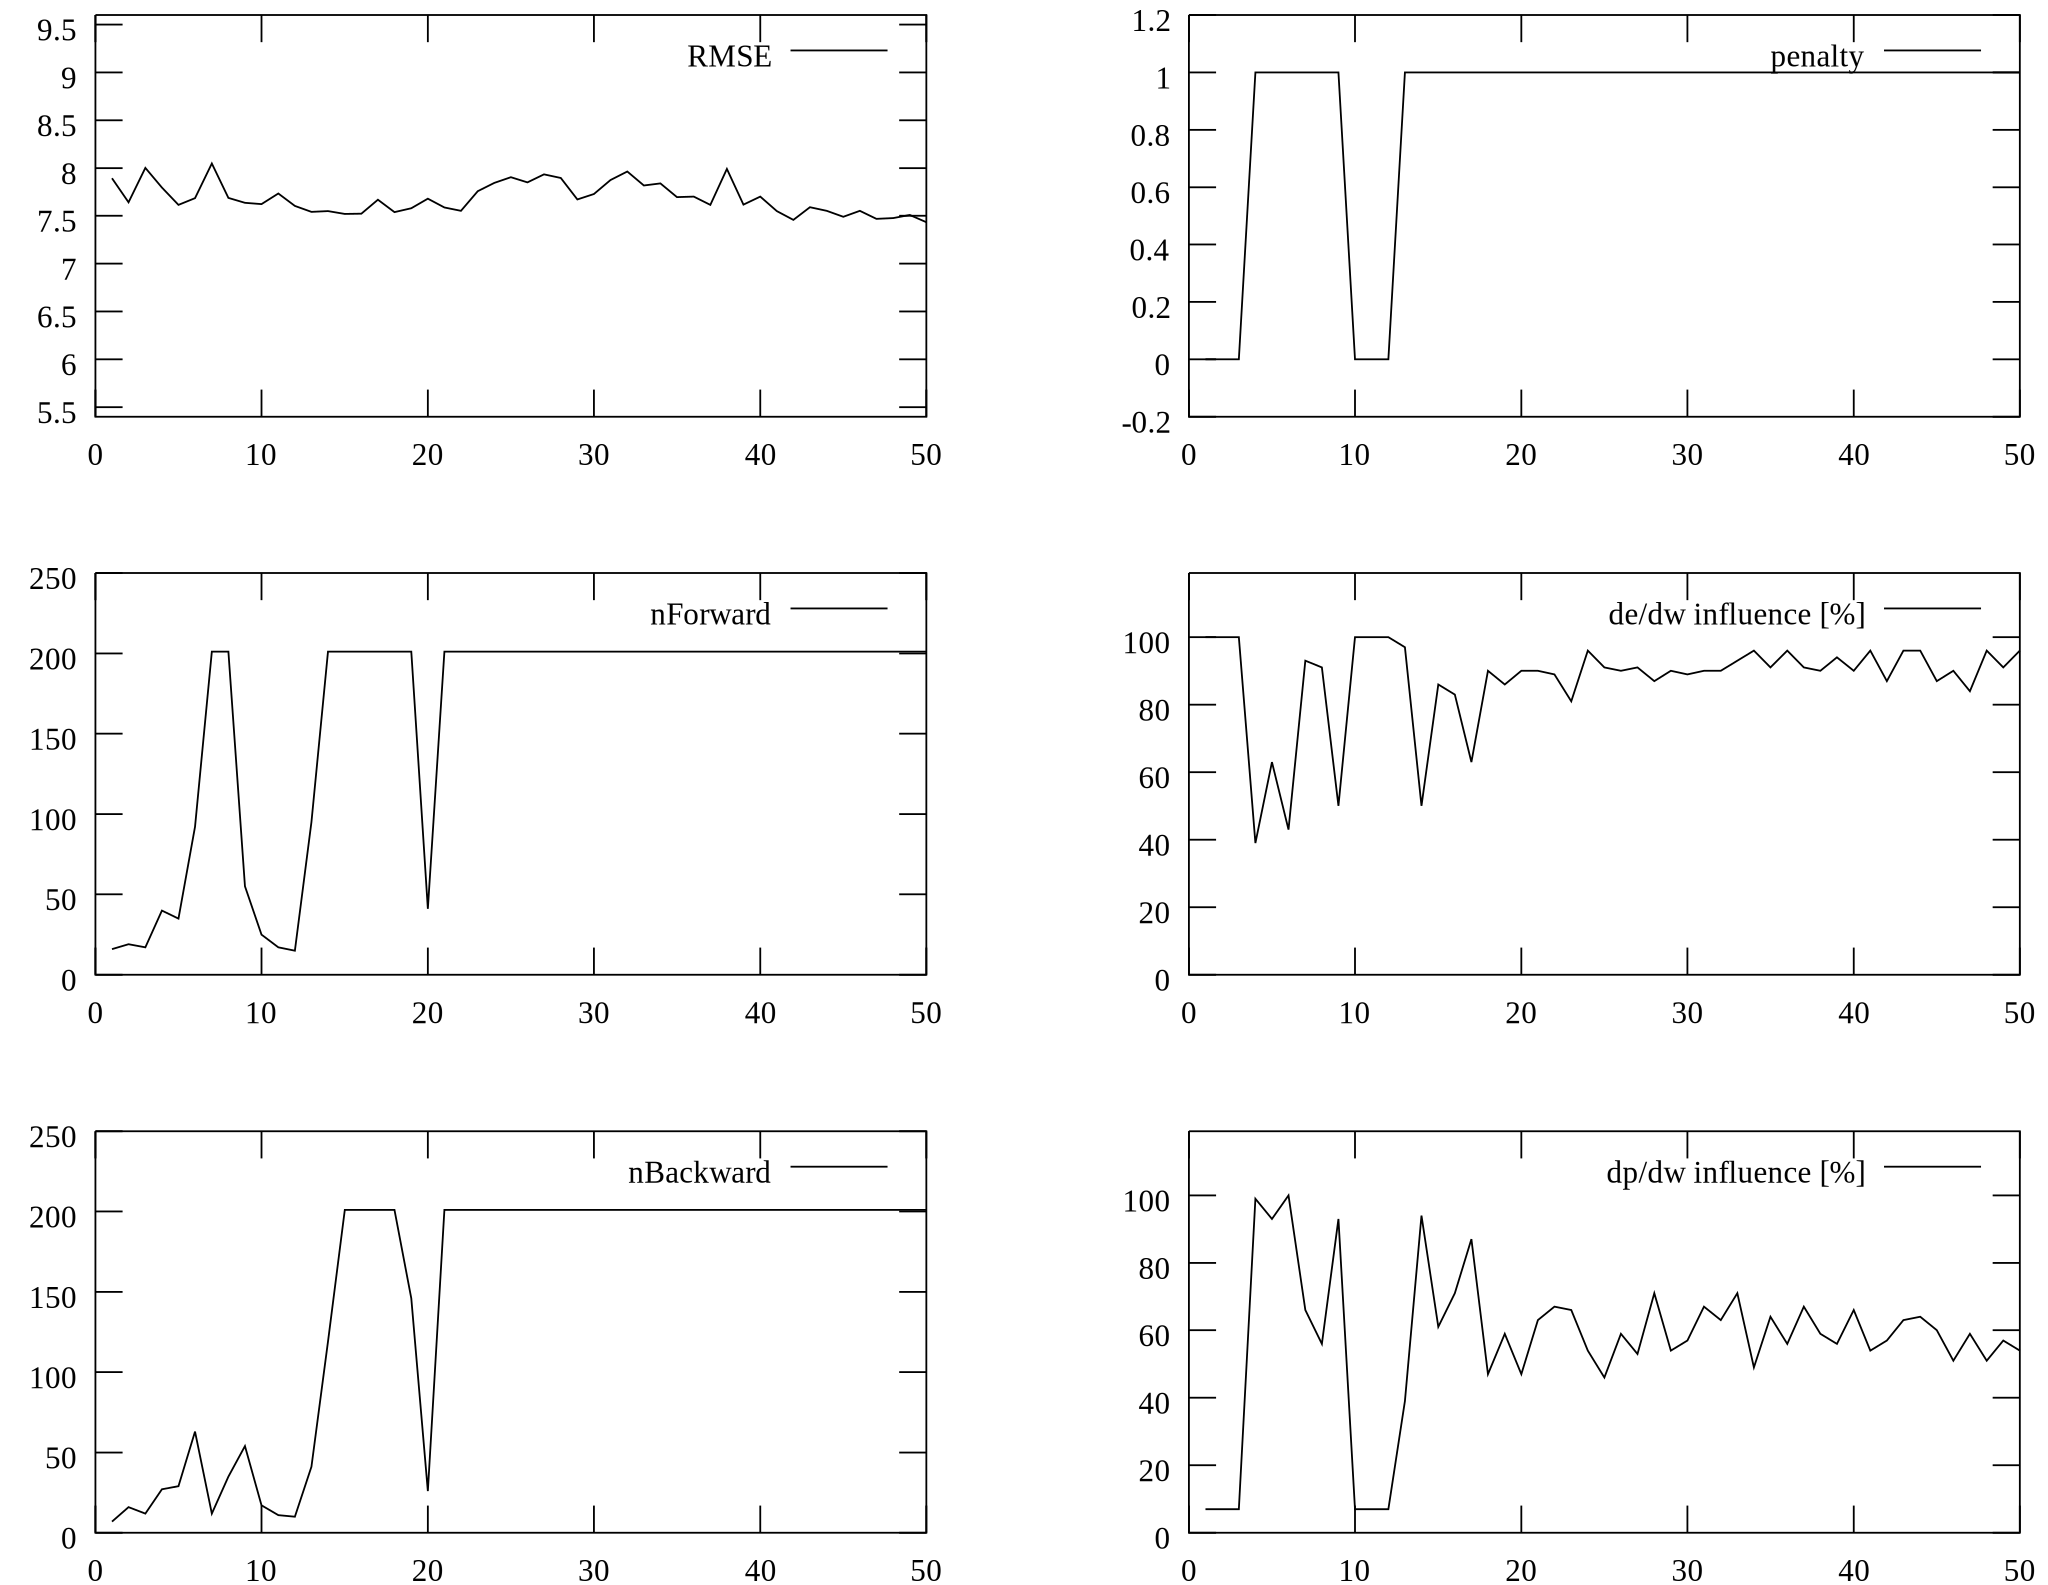
\includegraphics[scale=0.065]{img/gnn8}
\end{frame}

\begin{frame}
\frametitle{Eksperyment 2a : wpływ parametrów GNN}
\begin{itemize}
	\item Wykrywanie podgrafu
	\item 6 węzłów, 3 węzły podgrafu
	\item 20 grafów
	\item jeden zestaw początkowych wartości wag
	\item $contractionConstant$ = 1.2, 0.9, 0.6
	\item $minStateDiff$ = 10e-08, 10e-07
	\item $minErrorDiff$ = $minStateDiff$
	\item wybrana sieć nr 5 z poprzedniego eksperymentu
\end{itemize}
\end{frame}

\begin{frame}
	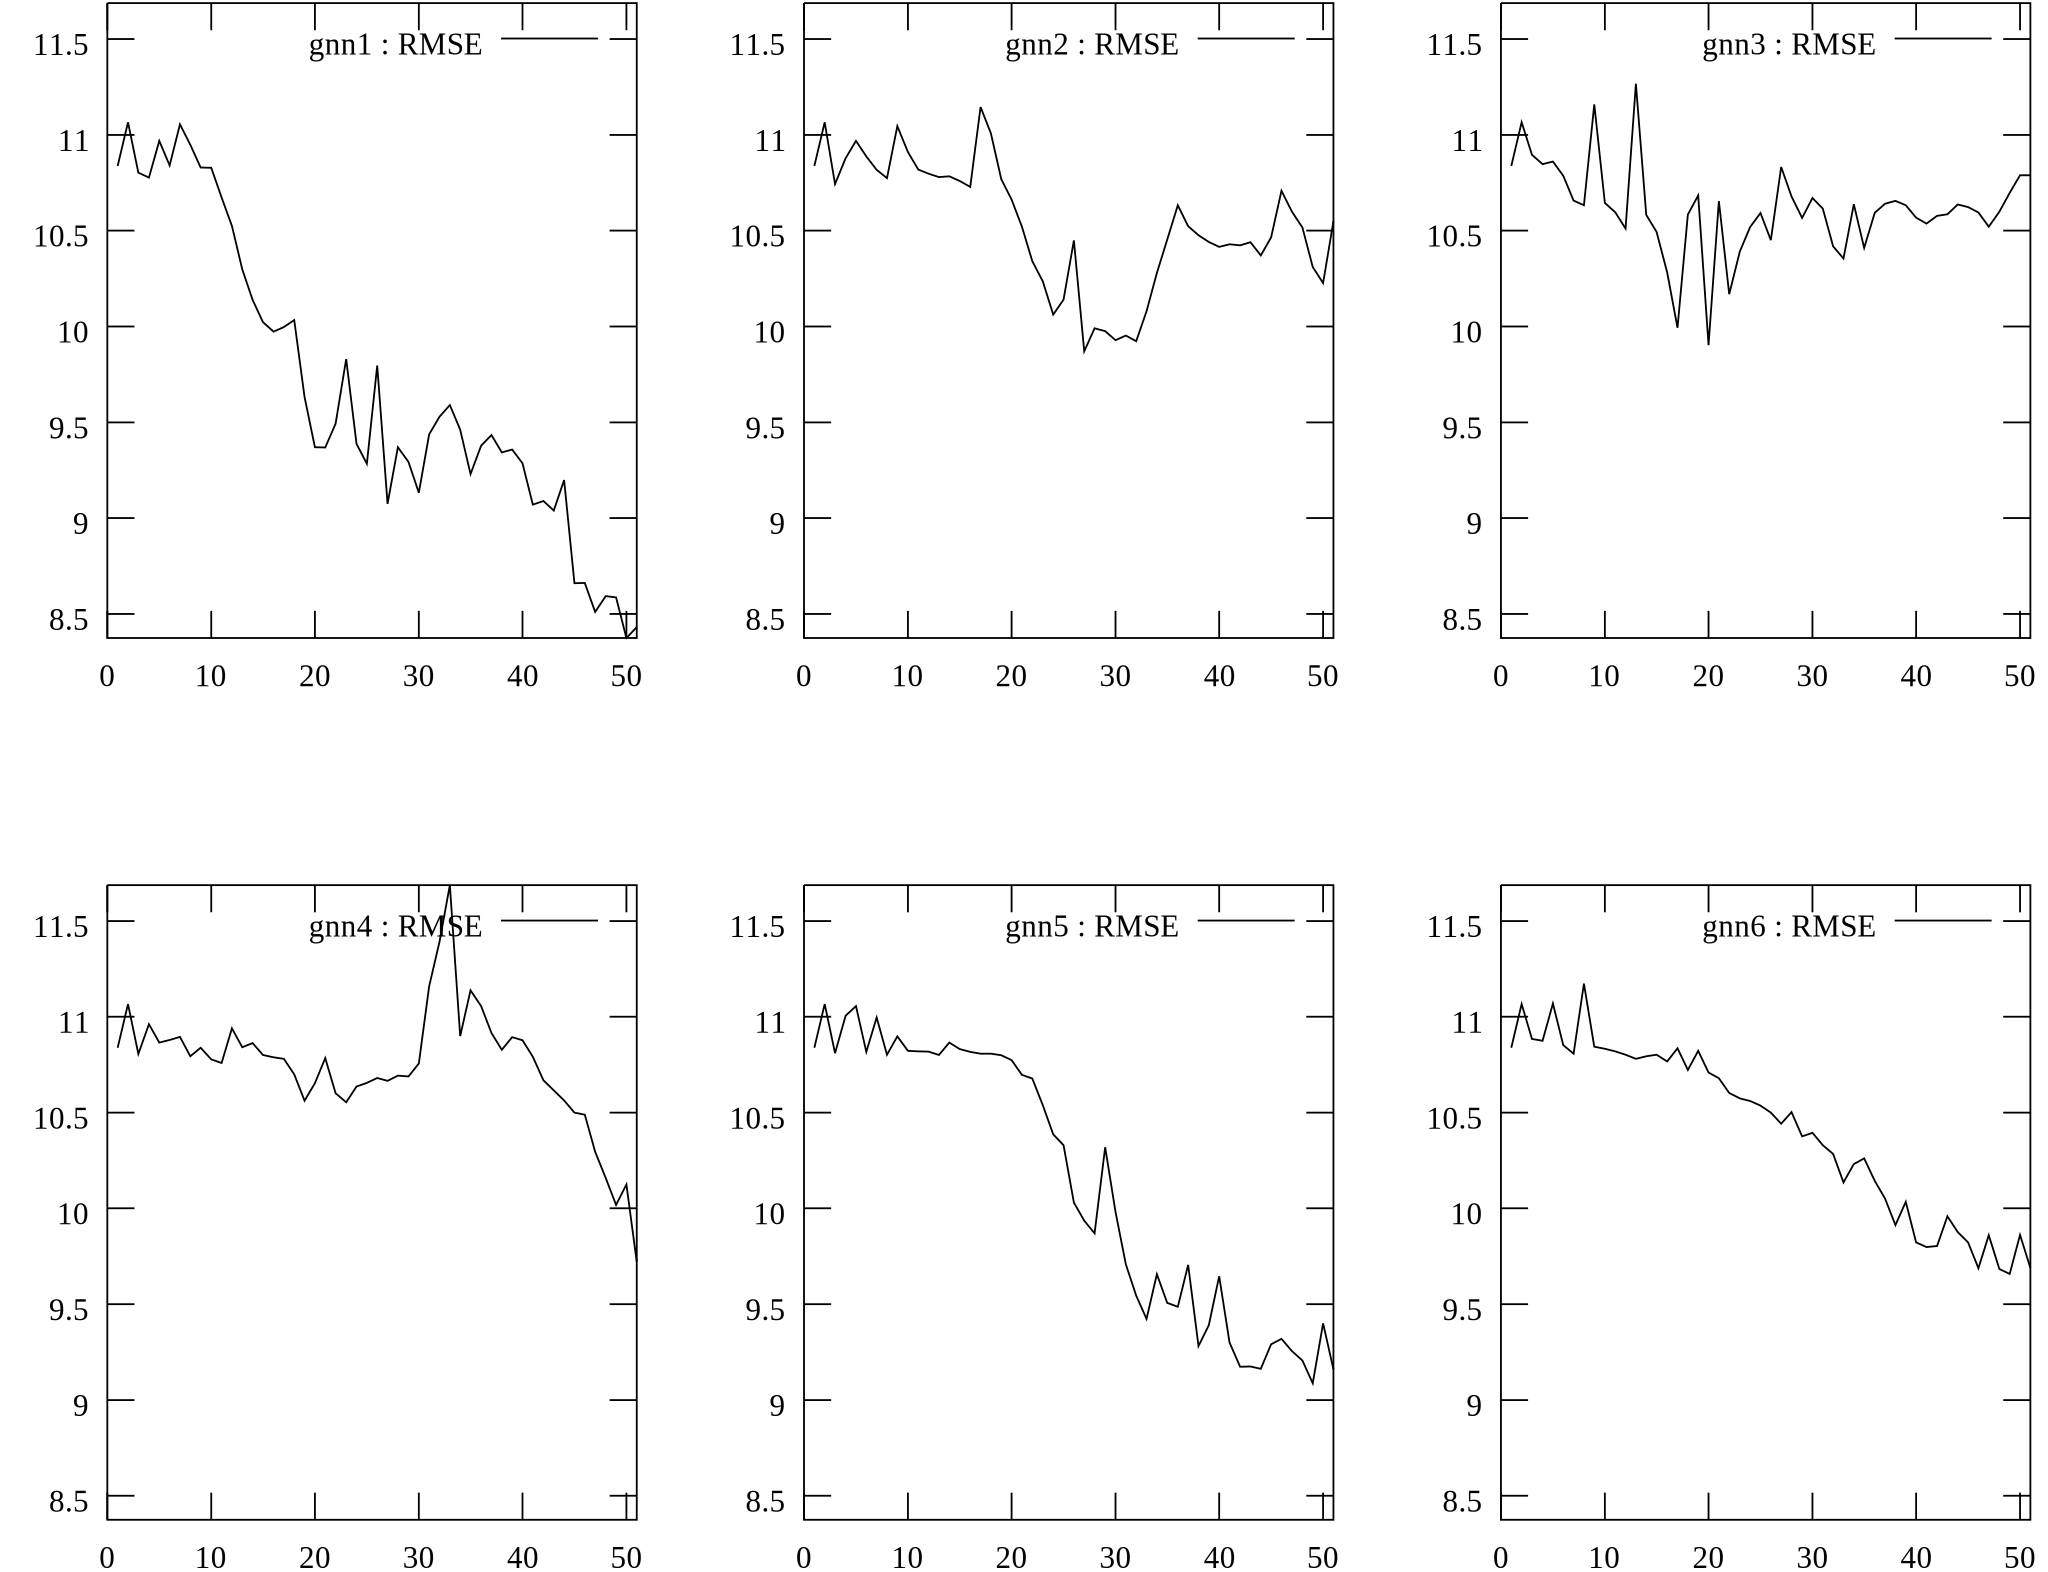
\includegraphics[scale=0.065]{img/rmse1}
\end{frame}
\begin{frame}
	\includegraphics[scale=0.065]{img/gnn1_1}
\end{frame}
\begin{frame}
	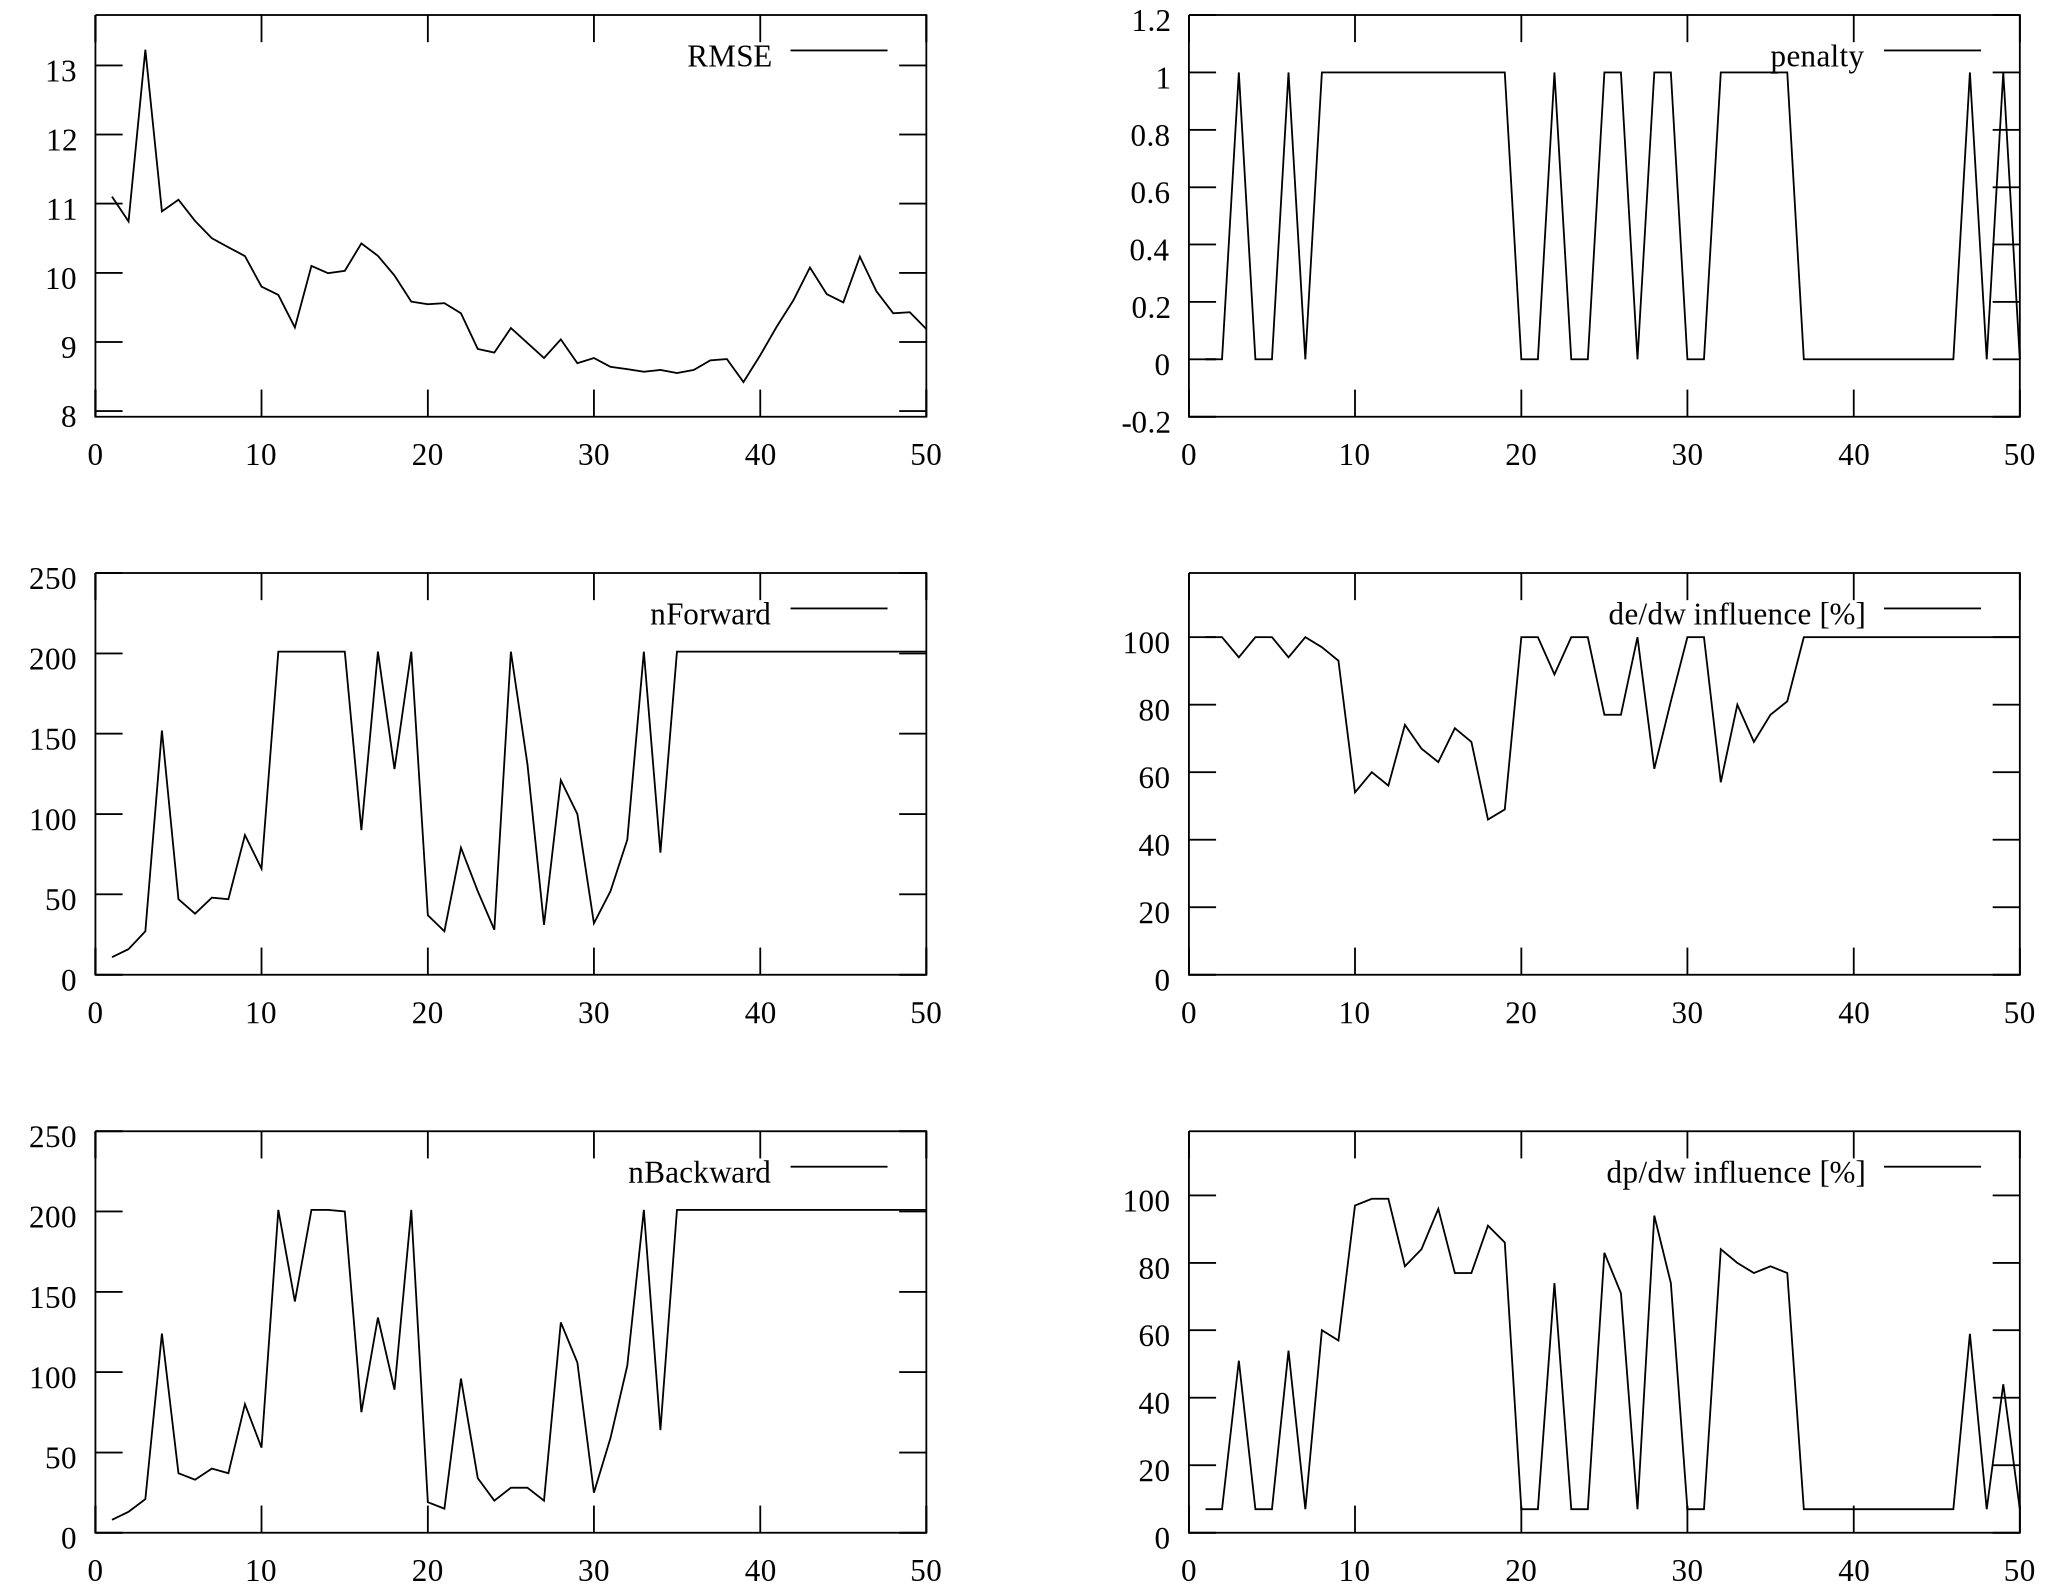
\includegraphics[scale=0.065]{img/gnn1_2}
\end{frame}
\begin{frame}
	\includegraphics[scale=0.065]{img/gnn1_3}
\end{frame}

\begin{frame}
\frametitle{Eksperyment 2b : wpływ parametrów GNN}
\begin{itemize}
	\item 20 grafów
	\item jeden zestaw początkowych wartości wag
	\item $contractionConstant$ = 1.2, 0.9, 0.6
	\item $minStateDiff$ = 10e-08, 10e-07
	\item $minErrorDiff$ = $minStateDiff$
	\item wybrana sieć nr 7 z poprzedniego eksperymentu
\end{itemize}
\end{frame}

\begin{frame}
	\includegraphics[scale=0.065]{img/rmse}
\end{frame}
\begin{frame}
	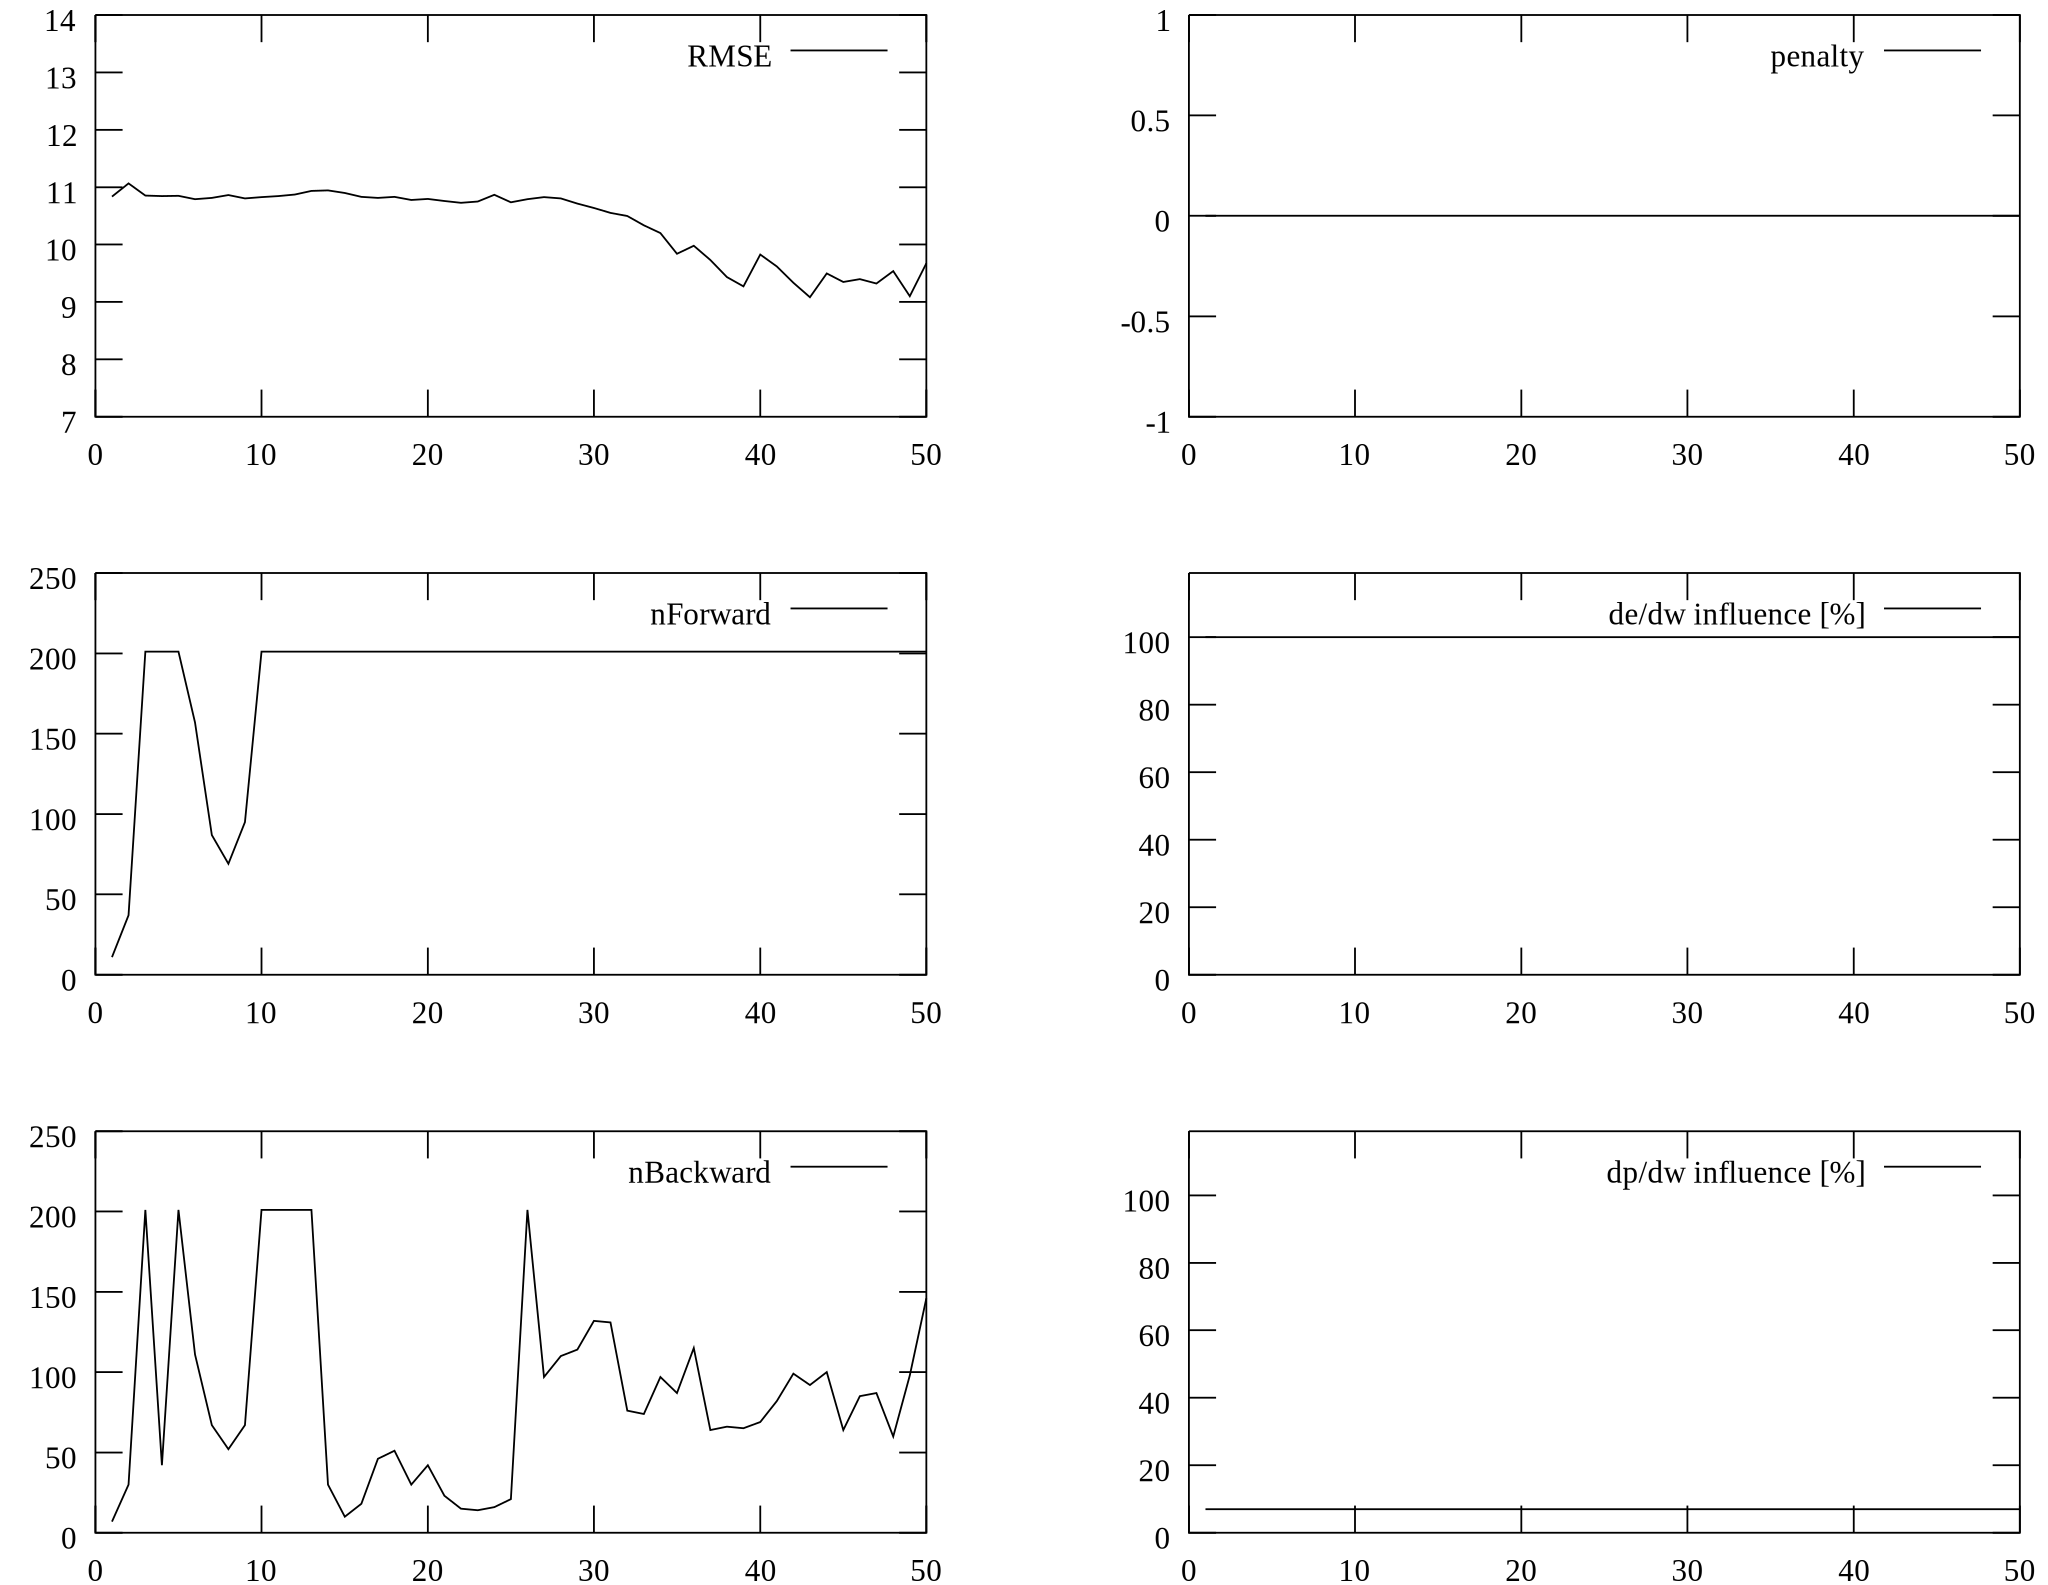
\includegraphics[scale=0.065]{img/params_set1}
\end{frame}
\begin{frame}
	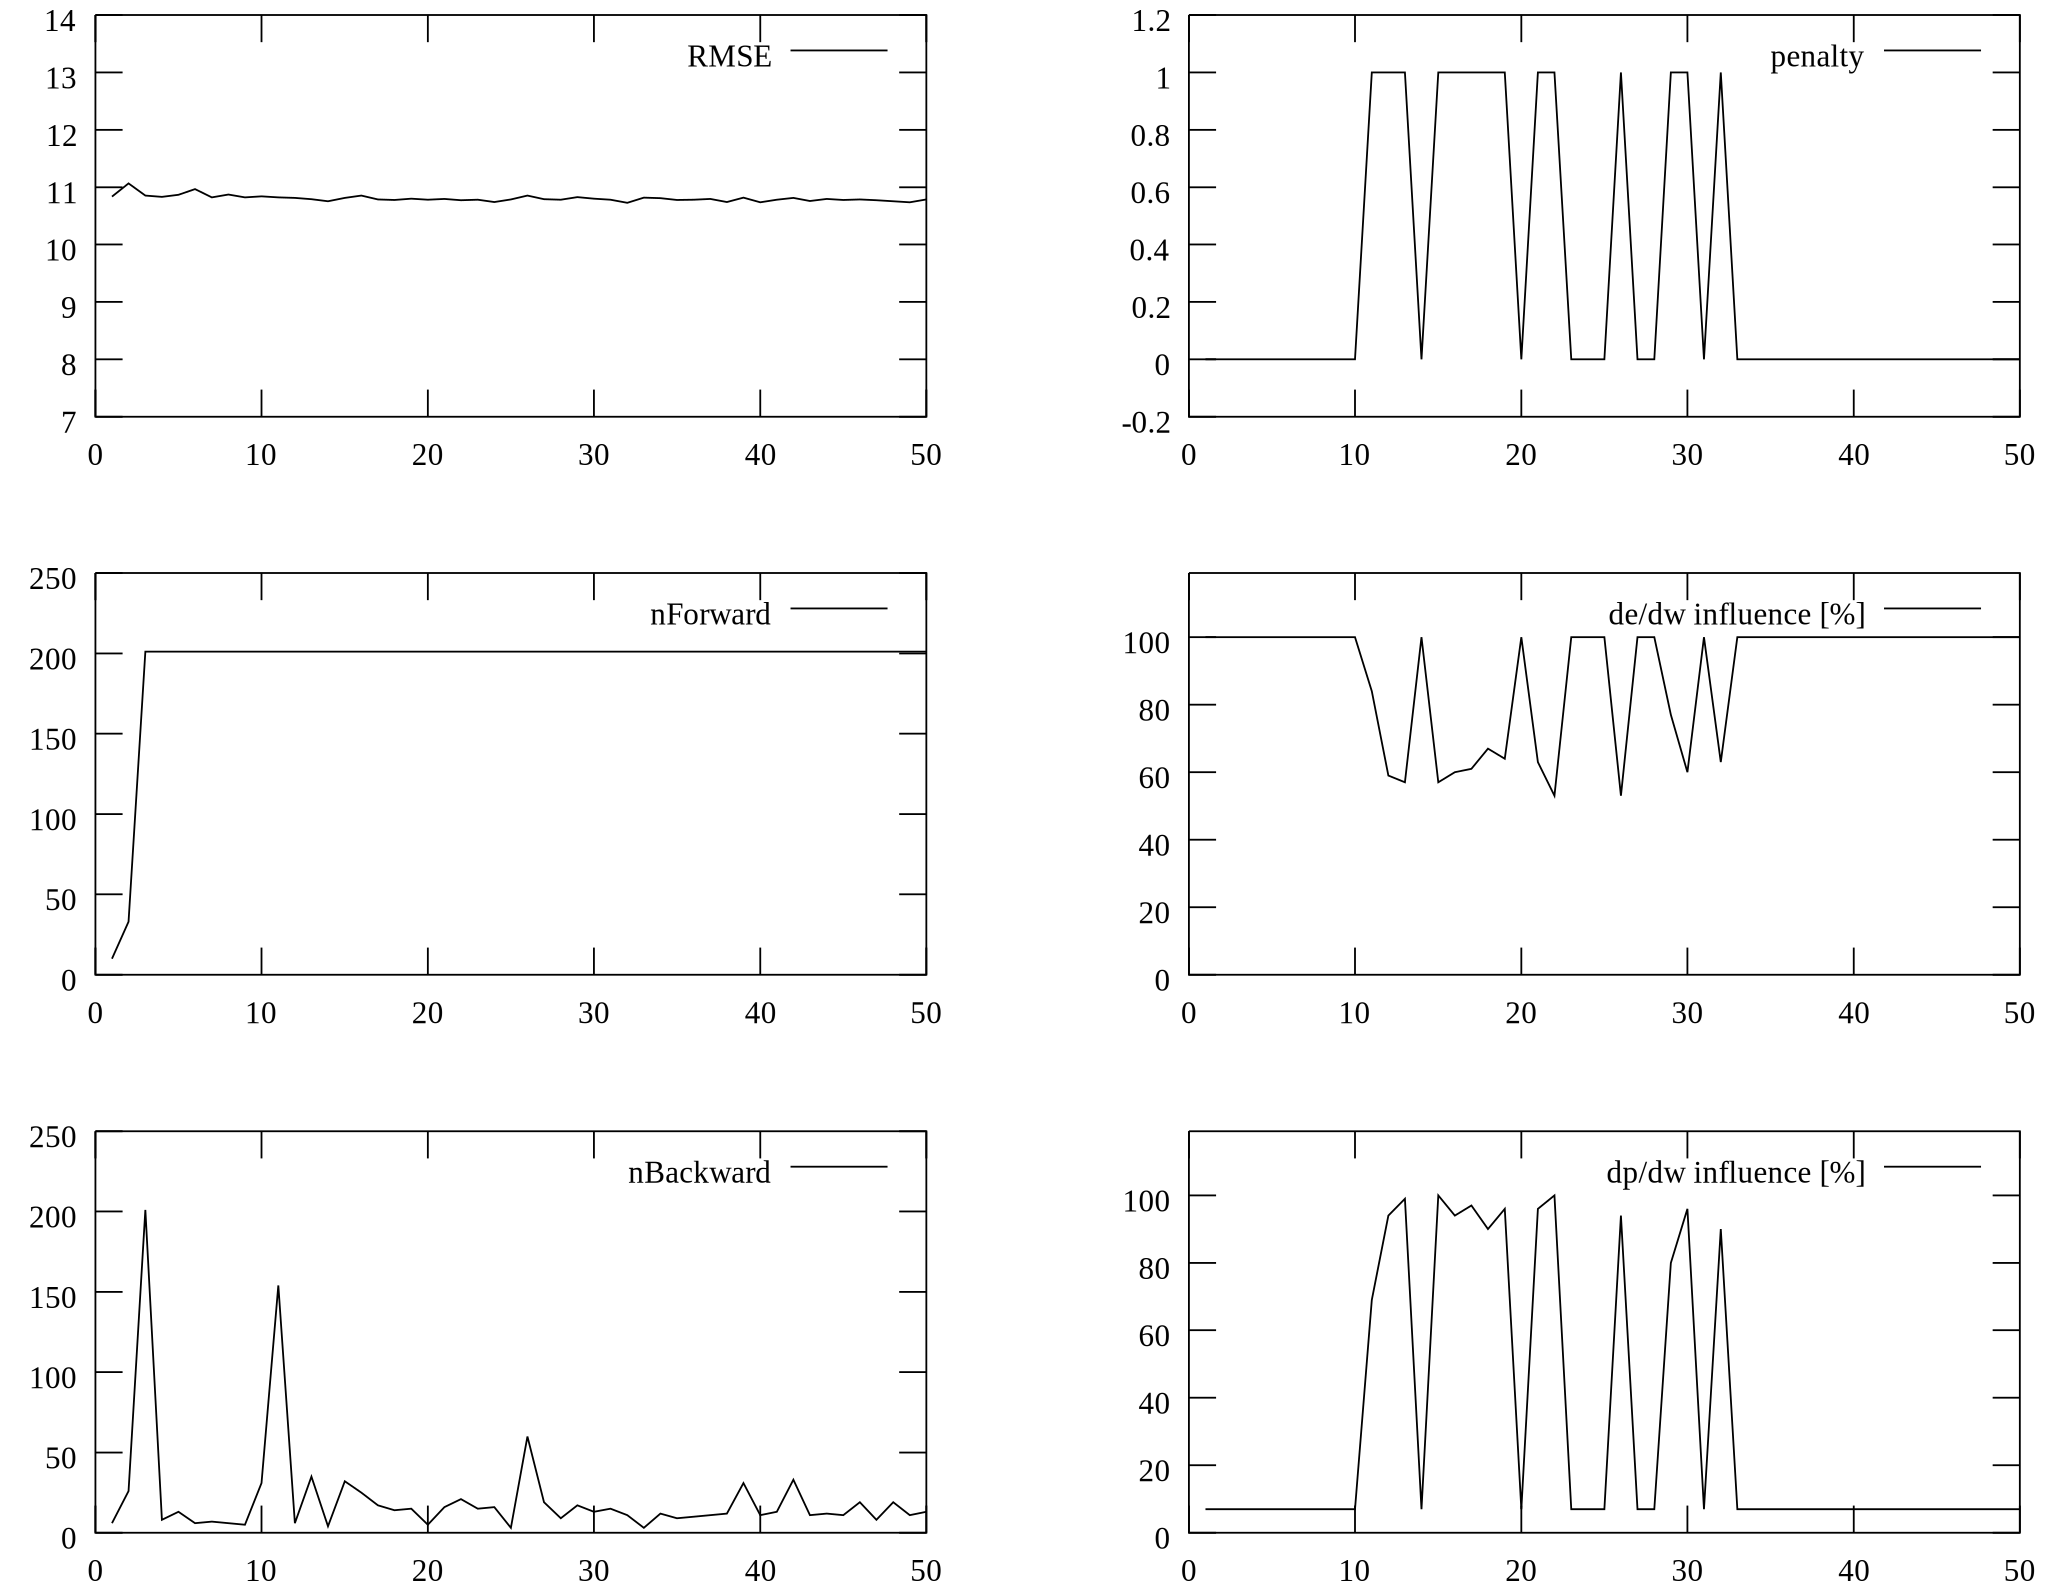
\includegraphics[scale=0.065]{img/params_set2}
\end{frame}
\begin{frame}
	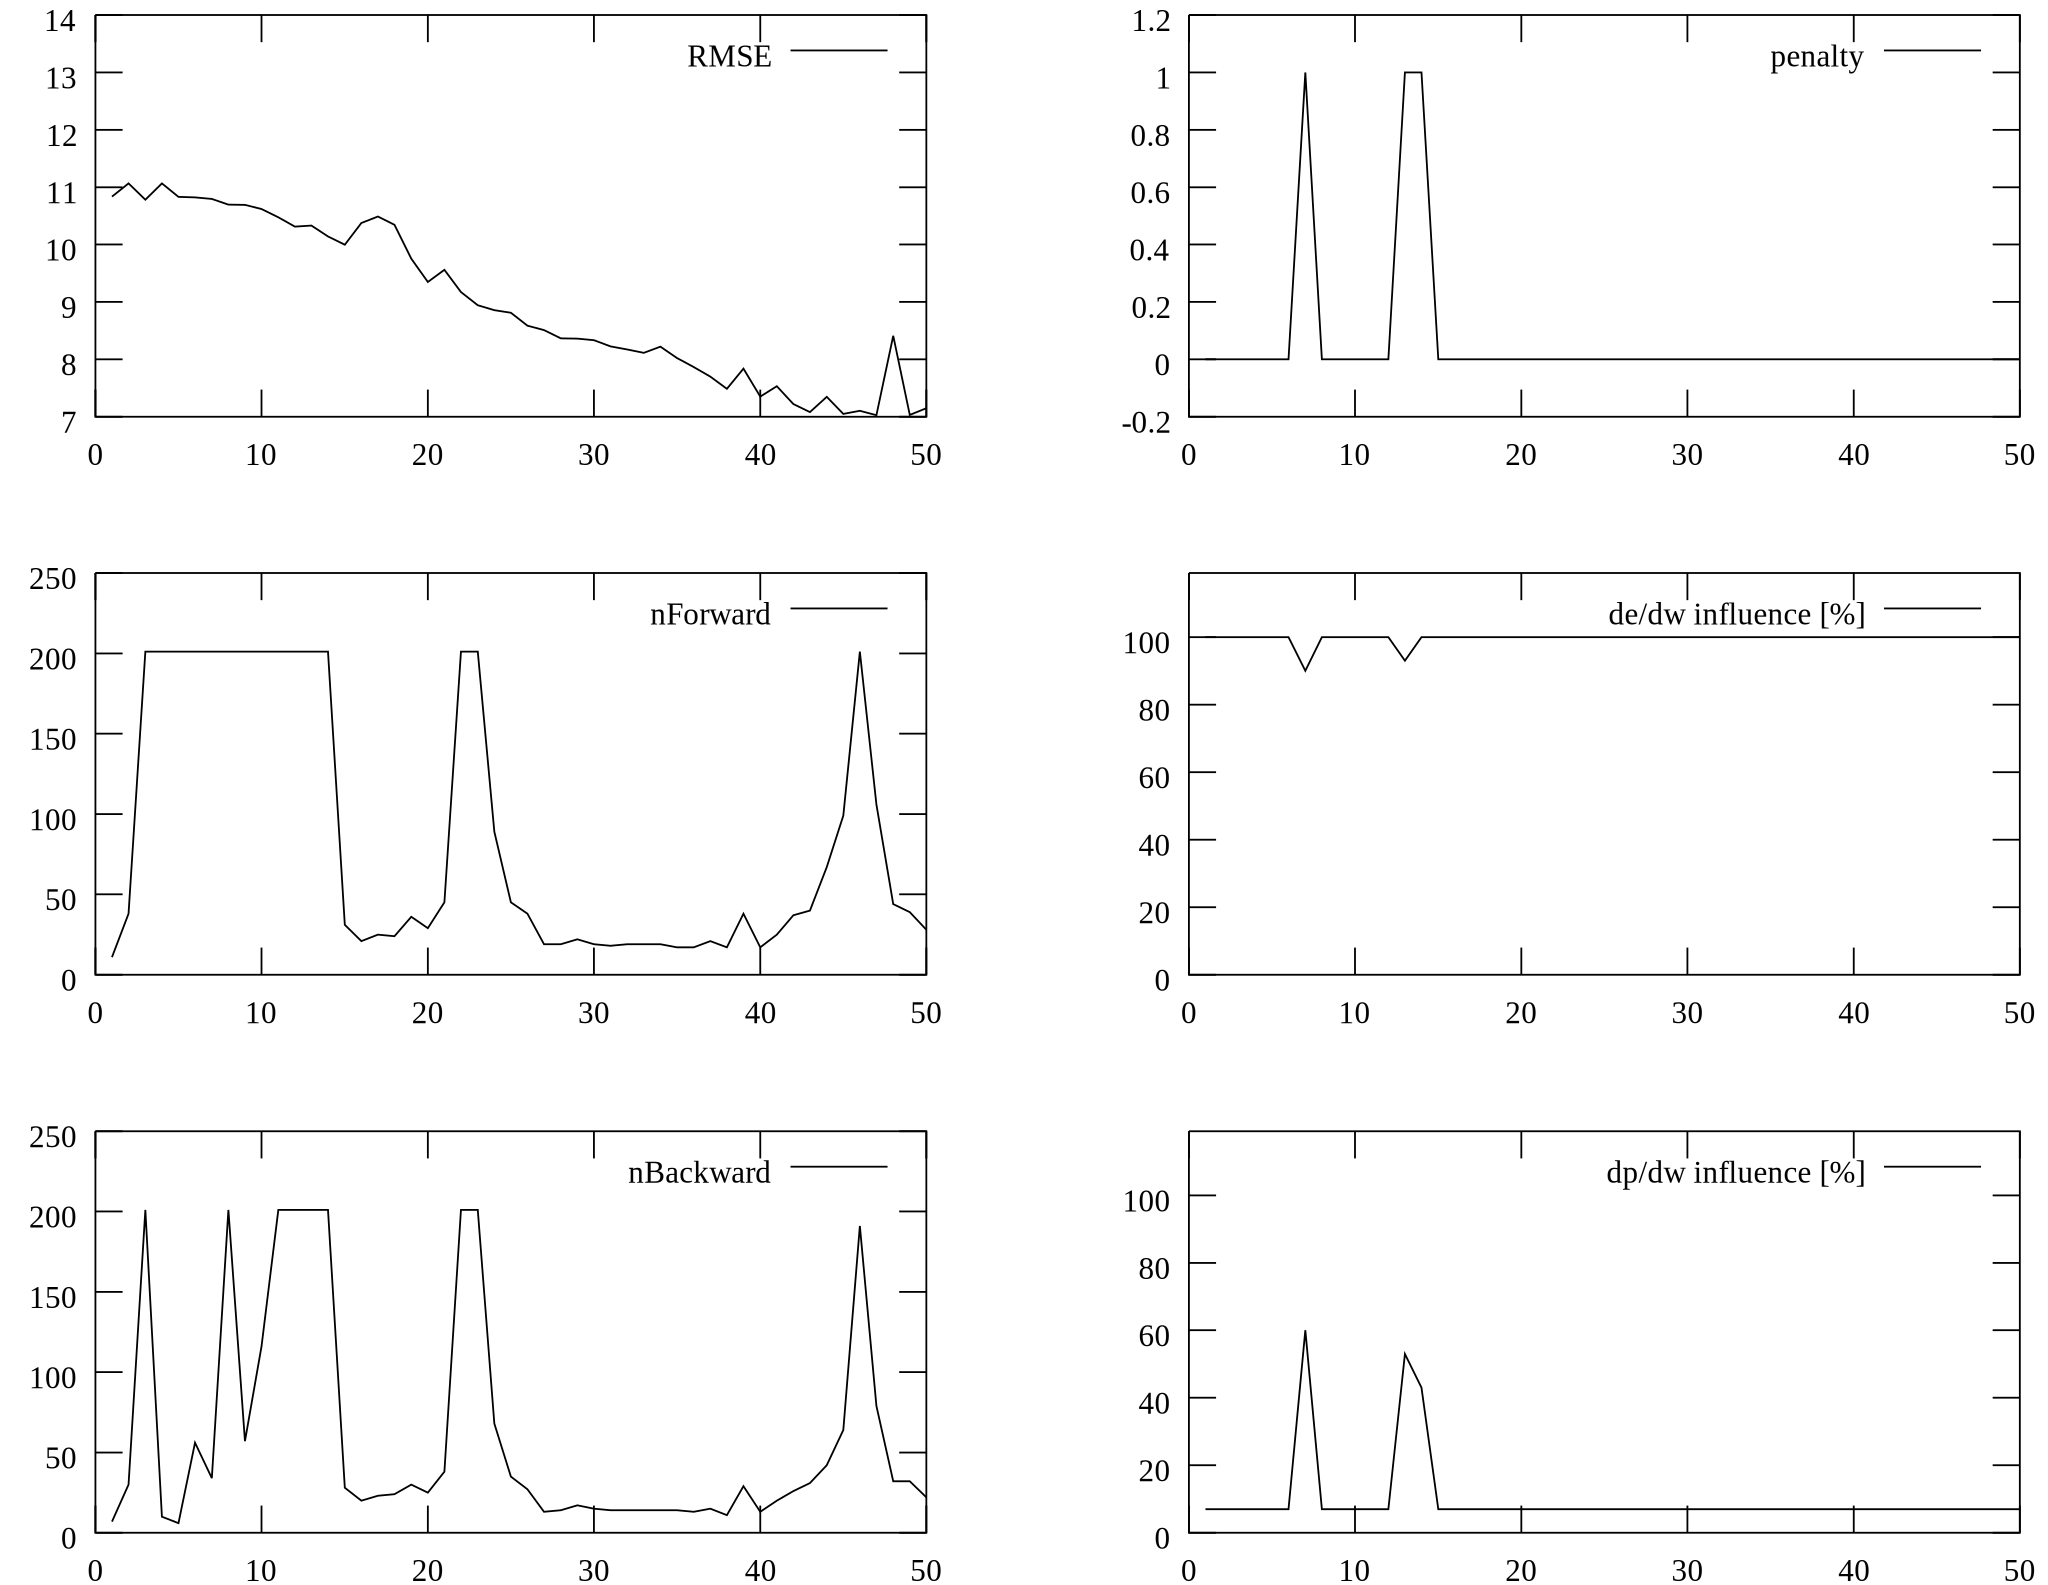
\includegraphics[scale=0.065]{img/params_set3}
\end{frame}
\begin{frame}
	\includegraphics[scale=0.065]{img/params_set4}
\end{frame}
\begin{frame}
	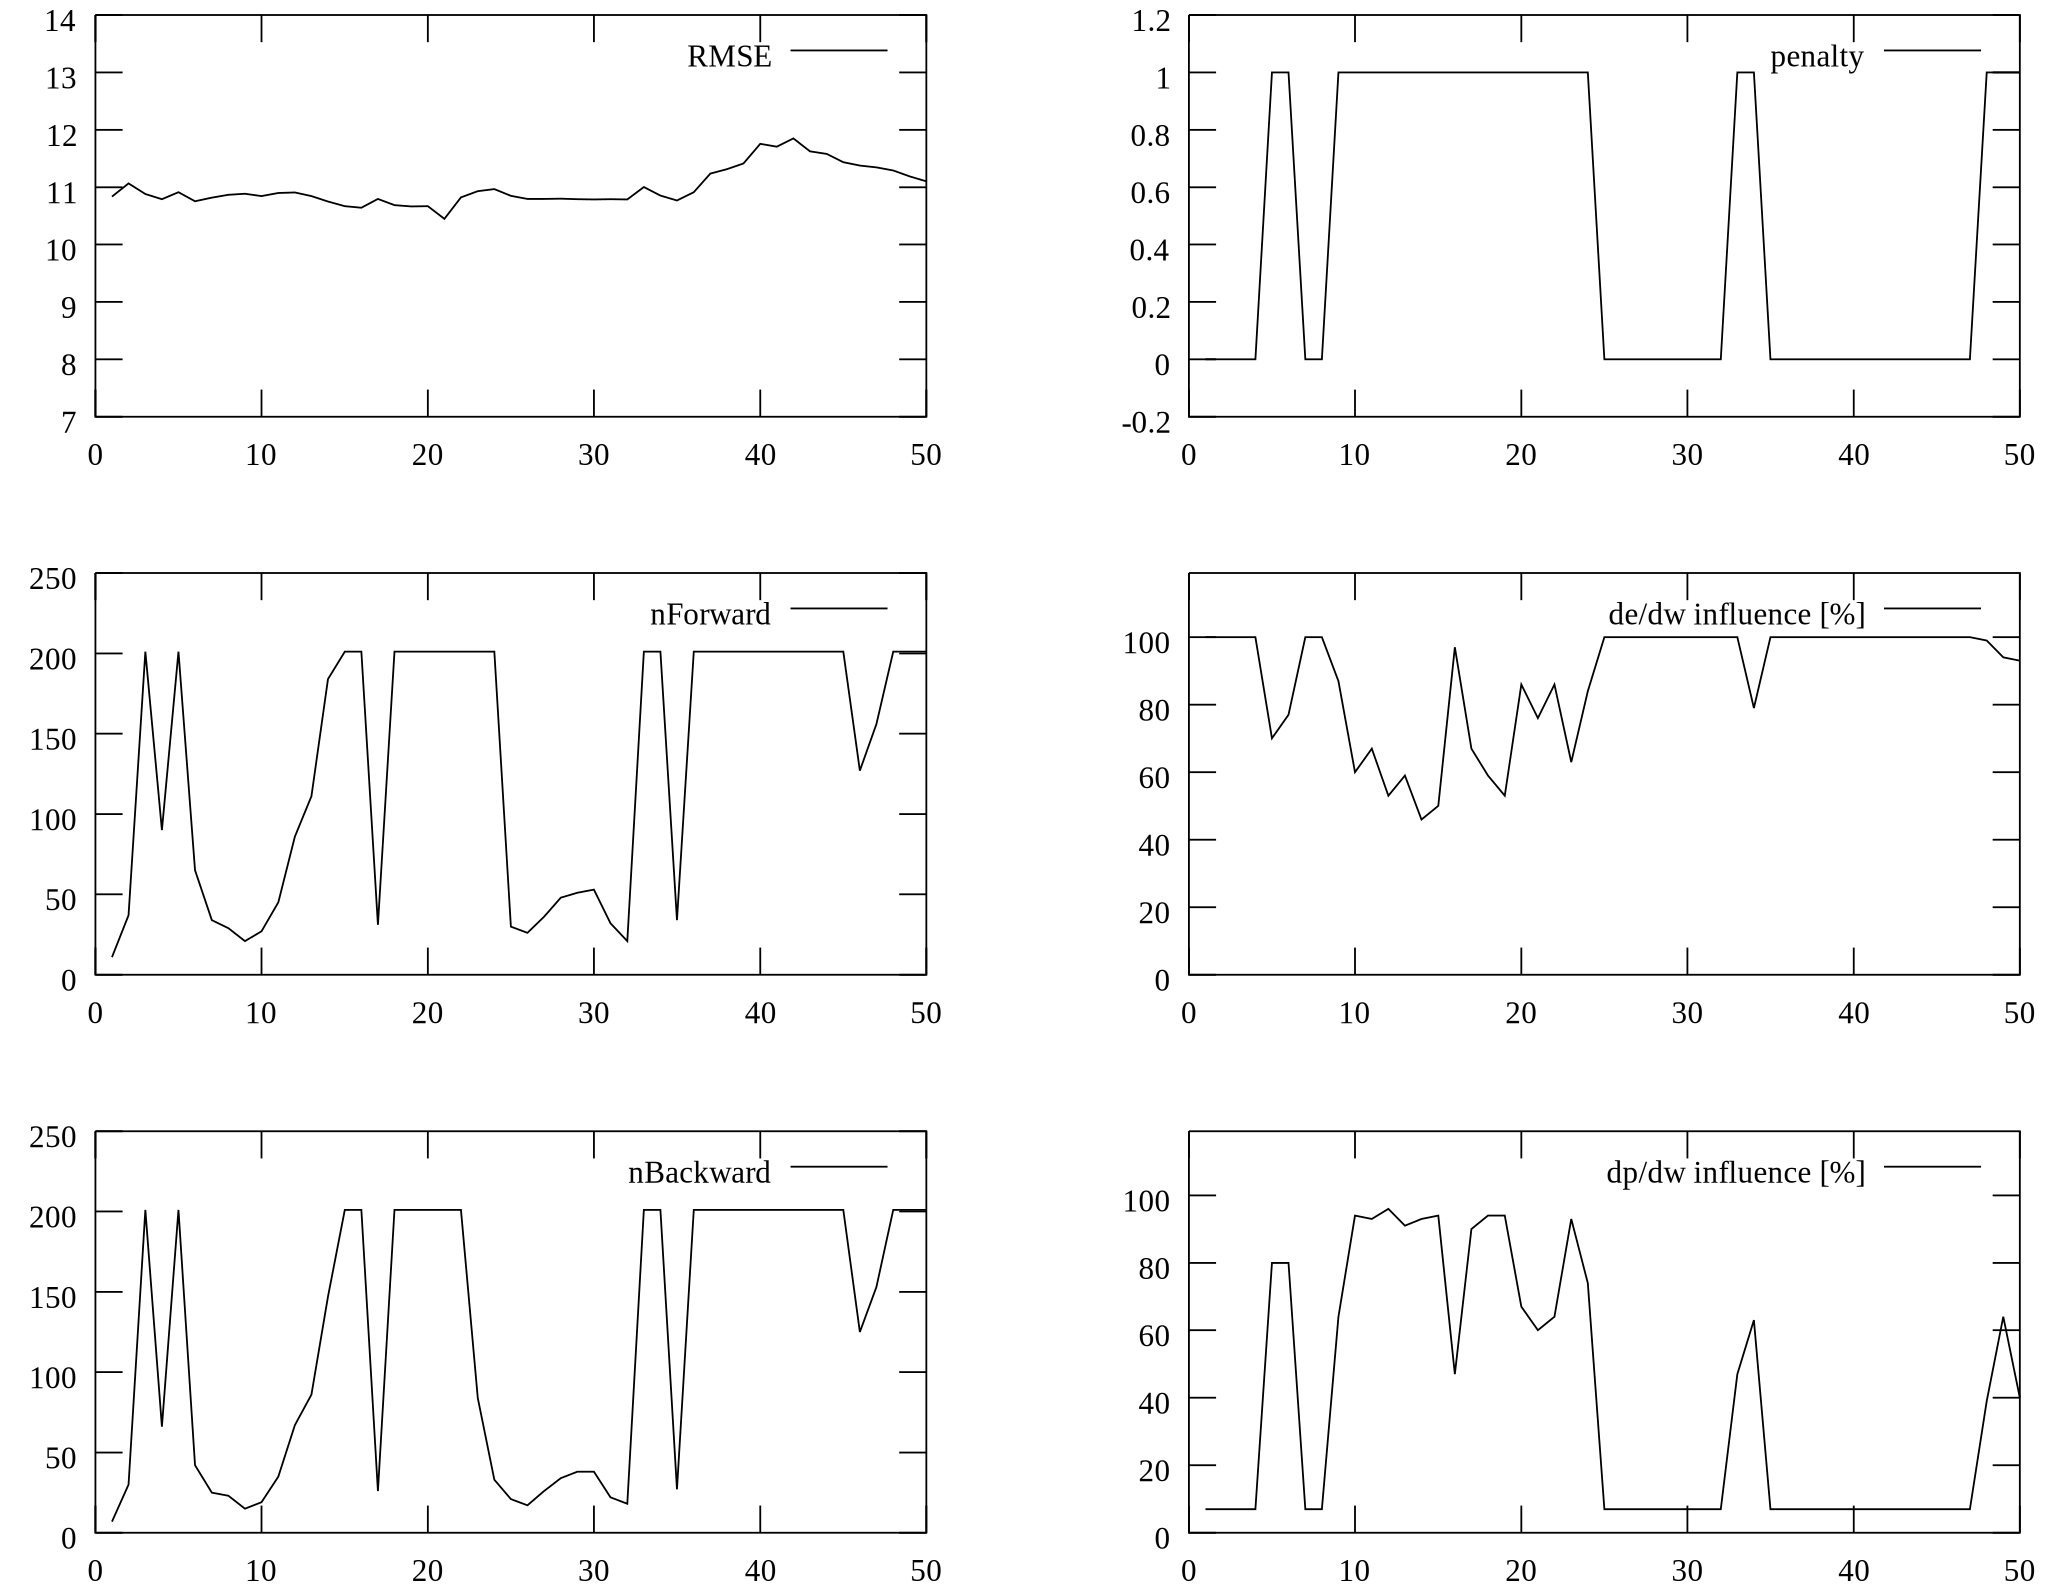
\includegraphics[scale=0.065]{img/params_set5}
\end{frame}
\begin{frame}
	\includegraphics[scale=0.065]{img/params_set6}
\end{frame}

\begin{frame}
\frametitle{Klasyfikacja węzłów - wyniki}
\setlength{\tabcolsep}{2pt}
\begin{table}[h!]
	\begin{center}
	\begin{tabular}{lrrrrr}
	\toprule
	& accuracy & precision & recall \\
	\midrule
	TR - średnia 	& 79\% & 83\% & 79\% \\
	TR - std 		& 8\% & 4\% & 14\% \\
	TST - średnia	& 75\% & 76\% & 81\% \\
	TST - std		& 8\% & 10\% & 14\% \\
	\bottomrule
	\end{tabular}
	\caption{5-krotna walidacja krzyżowa, najlepsza sieć z 10ciu, 200 iteracji}
	\end{center}
\end{table}
\end{frame}

\begin{frame}
\frametitle{Klasyfikacja węzłów - 100 grafów}
\setlength{\tabcolsep}{2pt}
\begin{table}[h!]
	\begin{center}
	\begin{tabular}{lrrrrr}
	\toprule
	& accuracy & precision & recall \\
	\midrule
	GNN - TR	&	90\% & 88\% & 95\% \\
	GNN - TST	&	87\% & 84\% & 95\% \\
	\midrule
	FNN - TR	&	96\% & 94\% & 100\% \\
	FNN - TST	&	97\% & 95\% & 100\% \\
	\bottomrule
	\end{tabular}
	\caption{Klasyfikacja węzłów 100 iteracji}
	\end{center}
\end{table}
\begin{itemize}
	\item zbiór uczący : 80 grafów
	\item zbiór testowy : 20 grafów
	\item wykorzystana GNN nr 5 z eksperymentu 1 (najlepsza)
	\item wykorzystana do porównania FNN z 5 neuronami ukrytymi
\end{itemize}
\end{frame}
\begin{frame}
	\includegraphics[scale=0.065]{img/80graphs}
\end{frame}

\begin{frame}
\frametitle{Wyniki - zbiór danych}
\begin{itemize}
	\item 14 węzłów, 7 węzłów podgrafu
	\item 100 grafów
	\item 1031 spośród 1400 węzłów posiada etykiety należące do podgrafu
	\item 702 spośród 1031 węzłów należy do podgrafu
	\item FNN : najlepsza z 10ciu, 5-krotna walidacja krzyżowa
	\item GNN : losowa sieć, 5-krotna walidacja krzyżowa, 50 iteracji
\end{itemize}
\end{frame}

\begin{frame}
\frametitle{Wyniki}
\setlength{\tabcolsep}{2pt}
\begin{table}[h!]
	\begin{center}
	\begin{tabular}{llll}
	\toprule
	& accuracy & precision & recall \\
	\midrule
	FNN - tr &	71\% &  65\% & 93\% \\
	FNN - tst &	71\% &  64\% &  93\% \\
	GNN - tr &	91\% &  87\%&  97\% \\
	GNN - tst &	91\% &  86\% &  97\% \\
	\bottomrule
	\end{tabular}
	\caption{Średnie wartości na zbiorze uczącym i testowym}
	\end{center}
\end{table}

\begin{table}[h!]
	\begin{center}
	\begin{tabular}{llll}
	\toprule
	& accuracy & precision & recall \\
	\midrule
	FNN - tr &	0.34\% &  0.67\% & 1.86\% \\
	FNN - tst &	2.45\% &  1.73\% &  2.93\% \\
	GNN - tr &	1.62\% &  1.71\% &  2.07\% \\
	GNN - tst &	3.06\% &  3.70\% &  1.39\% \\
	\bottomrule
	\end{tabular}
	\caption{Odchylenia standardowe}
	\end{center}
\end{table}
\end{frame}

\begin{frame}
\frametitle{Wnioski}
\begin{itemize}
	\item Najlepszy efekt przy zachowaniu kontrakcji
	\item Brak zbieżności kontrakcji – brak poprawy
	\item Balansowanie na granicy zbieżności / ograniczona ilość kroków obliczenia stanu i błędu dopuszczalne
	\item Należy unikać nakładania niepotrzebnie kary kontrakcji
	\item Można dobrać zestaw parametrów (i początkowych wag) na podzbiorze danych
\end{itemize}
\end{frame}

\end{document}
